%%%%%%%%%%%%%%%%%%%%%%%%%%%%%%%%%%%%%%%%%%%%%%%%%
%------ LaTeX-Template
%%%%%%%%%%%%%%%%%%%%%%%%%%%%%%%%%%%%%%%%%%%%%%%%%

%---- Header (mit Formateinstellugen) laden, Inputencoding prüfen ------

%%%%%%%%%%%%%%%%%%%%%%%%%%%%%%%%%%%%%%%%%%%%%%%%%
%---- LaTeX-Header
%%%%%%%%%%%%%%%%%%%%%%%%%%%%%%%%%%%%%%%%%%%%%%%%%

\documentclass[12pt,paper=A4,numbers=noenddot,bibliography=totoc,listof=totoc,DIV=11,BCOR=1mm]{scrreprt}
%  Bindekorrektur BCOR (verlorener Rand am linken Blattrand)! Wert haengt von der Art der Heftung ab!!
%  Satzspiegeleinstellung DIV von KOMA-Script / sccreprt.

\pagestyle{headings}

\usepackage[T1]{fontenc} % Font Encoding fuer europaeische Schriften mit Umlauten (Unterstuetzung der Worttrennung)
\usepackage{lmodern} % PostScript-Varianten der TeX Computer Modern-Schriften laden
\usepackage[english,ngerman]{babel} % Spracheinstellungen fuer Englisch und Neudeutsch laden

\usepackage{setspace}

\usepackage{graphicx} % Grafikeinbindung (fuer .JPG, .JPEG, .PNG und .PDF, falls pdflatex benutzt wird)
\usepackage[table]{xcolor} % ermoeglicht farbige Schrift und farbige Tabellenzeilen
\definecolor{black}{gray}{0} % Umdefinition der Farbe black, falls noetig (0=schwarz, 1=weiss)
\definecolor{dblue}{rgb}{0.1,0.2,0.6} % Dunkelblau, fuer Hyperlinks
\definecolor{lgray}{gray}{0.9} % Hellgrau, fuer Tabellen (0=schwarz, 1=weiss)

\usepackage{booktabs} % fuer schoene Tabellen

\usepackage[round,authoryear]{natbib} % Literaturverweise mit Name/Jahreszahl in runden Klammern
\bibpunct[:\,]{(}{)}{,}{a}{}{,~}  % Feinformatierung der Natbib-Zitierweise

\usepackage[hyphens]{url}
\usepackage[colorlinks=true,linkcolor=black,citecolor=dblue,urlcolor=dblue]{hyperref} 
\usepackage{hyperref}  
% die Pakete url und hyperref ermoeglichen anklickbare URLs im Quellenverzeichnis in definierter Farbe, 
% sie ermoeglichen den Zeilenumbruch bei langen URLs, und sie erzeugen Hyperlinks (Farbe s.o.) 
% zwischen Quellenverweis und Quellenverzeichnis sowie zwischen label und ref im PDF-Dokument

\usepackage[section]{placeins}
% Fonteinstellungen fuer Bildunterschriften: Unterschrift serifenlos, "Abbildung" fett (bfseries = bold face series)
\setkomafont{captionlabel}{\sffamily\bfseries}
\setkomafont{caption}{\sffamily}

%------------------------------------------------------------------------------------------------------------------
%------ Eigenstaendigkeitserklaerung im gerahmten Kasten (parbox in einer framebox) ------
%------------------------------------------------------------------------------------------------------------------

\newcommand{\eigen}{
\setlength{\fboxsep}{2ex}
\setlength{\fboxrule}{0.8pt} 
% Einstellungen fuer Rahmenabstand und Rahmendicke der Framebox
\begin{center}
	\fbox{
		\parbox{0.8\linewidth}{
		Ich versichere, die vorliegende Arbeit selbstst\"andig ohne fremde Hilfe verfasst 
		und keine anderen Quellen und Hilfsmittel als die angegebenen benutzt zu haben. 
		Die aus anderen Werken w\"ortlich entnommenen Stellen oder dem Sinn nach 
		entlehnten Passagen sind durch Quellenangaben eindeutig kenntlich gemacht.
		\par\bigskip\bigskip\bigskip\bigskip
		\hspace*{0.8cm}Ort, Datum \hfill \vorname~\nachname\hspace*{0.8cm}
		}
	}
\end{center}
}

%%%%%%%%%%%%%%%%%%%%%%%%%%%%%%%%%%%%%%%%%%%%%%%%%

%\usepackage[applemac]{inputenc} % Inputencoding f�r Mac
%\usepackage[latin1]{inputenc} % Inputencoding f�r PC/Win
\usepackage[utf8]{inputenc} % Inputencoding, universell
%\usepackage[utf8x]{inputenc} % Inputencoding, universell


%------------------------ Titelblatt-Layout laden ----------------------------------

%%%%%%%%%%%%%%%%%%%%%%%%%%%%%%%%%%%%%%%%%%%%%%%%%
%------ LaTeX-Titelblatt
%------ Deklarationen fuer die Titelseite
%%%%%%%%%%%%%%%%%%%%%%%%%%%%%%%%%%%%%%%%%%%%%%%%%

\title{\titel\\[2ex]
\LARGE Bachelor-Thesis\\
\large zur Erlangung des akademischen Grades B.Sc.\\[1.5ex]
\LARGE \vorname~\nachname\\[0.5ex] 
\large \matrikelnummer
}

\author{\unitlength1mm
\large\raisebox{-1ex}{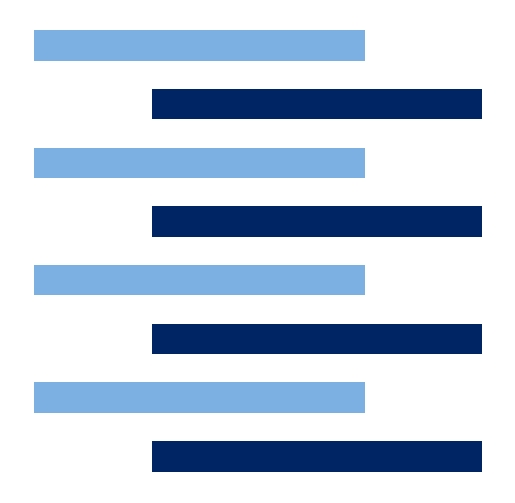
\includegraphics[width=4em]{HAW_wuerfel}}\hspace{1ex}
\parbox[b]{11.2cm}{\sffamily\large%
Hochschule für Angewandte Wissenschaften Hamburg\\[-0.2ex]
Fakultät Design, Medien und Information\\[-0.2ex]
Department Medientechnik
}\\[6ex]
\sffamily\large Erstprüfer: \erstpruef\\[0.5ex]
\sffamily\large Zweitprüfer: \zweitpruef}

%%%%%%%%%%%%%%%%%%%%%%%%%%%%%%%%%%%%%%%%%%%%%%%%%

%---------------------------- Titeldefinitionen --------------------------------------

\newcommand{\vorname}{Sebastian}
\newcommand{\nachname}{Bohn}
\newcommand{\matrikelnummer}{2036605}

\newcommand{\titel}{Analyse und Evaluierung von plattformübergreifenden Spiel-Engines und Frameworks,anhand der Implementierung einer mobilen Beispielapplikation}

\newcommand{\erstpruef}{Prof. Dr. Edmund Weitz}
\newcommand{\zweitpruef}{Prof. Dr. Andreas Plaß}

\date{vorläufige Fassung vom \today}   % Vorab-Version 
%\date{\sffamily Hamburg, DD. MM. YYYY}  % Abgabedatum!

%----------------------------- ANFANG --------------------------------------

\begin{document}
\selectlanguage{ngerman}
\setlength{\parindent}{0em}
% Titelseite erzeugen
\maketitle
% Inhaltsverzeichnis erzeugen          
\tableofcontents
% Seitenumbruch
\clearpage

%----------------------------INHALT---------------------------------------

%---------------------------ABSTRACT------------------------------------

\thispagestyle{empty}
\selectlanguage{english}
\section*{\centering\abstractname}

%TODO: English abstract

\selectlanguage{ngerman}
\section*{\centering\abstractname}

%TODO: Deutsches abstract

%----------------------------TEXT-----------------------------------------------

%TODO: Kapitel 1
\chapter{Einleitung}

\section{Motivation}
\section{Gliederung}

%Kapitel 2
\chapter{Mobile Systeme}
%TODO Einleitung Kapitel

\section{Marktanalyse zur Gewichtung der mobilen Systeme und der Applikationen}
Welche mobilen Systeme derzeit am meisten gefragt und verbreitet sind, soll in diesem Abschnitt analysiert werden. Dieses Wissen ist nötig, um vor dem Entwicklungsprozess die erfolgreichsten und erfolgversprechendsten Plattformen auszuwählen und miteinzubeziehen.
Weiterhin soll geklärt werden wie viele Applikationen diese Plattformen in ihren Stores bereitstehen und wie die Kategorien gewichtet sind.

\subsection{Marktanteile der mobilen Betriebssysteme}
\label{subsec:Marktanteile_mobile_Systeme}
Eine Statistik über die Marktanteile der mobilen Betriebssysteme bei Smartphones, soll veranschaulichen welche Systeme aktuell zu den führenden gehören. Zusätzlich wird eine zukünftige Verteilung prognostiziert. Die Darstellungen beziehen sich auf Daten der International Data Corporation (IDC), über den globalen Absatz von Smartphones und wurde im August 2015 veröffentlicht. (Abb. \ref{graph_mobile_systems})

\begin{figure}[htbp]
	\centering
	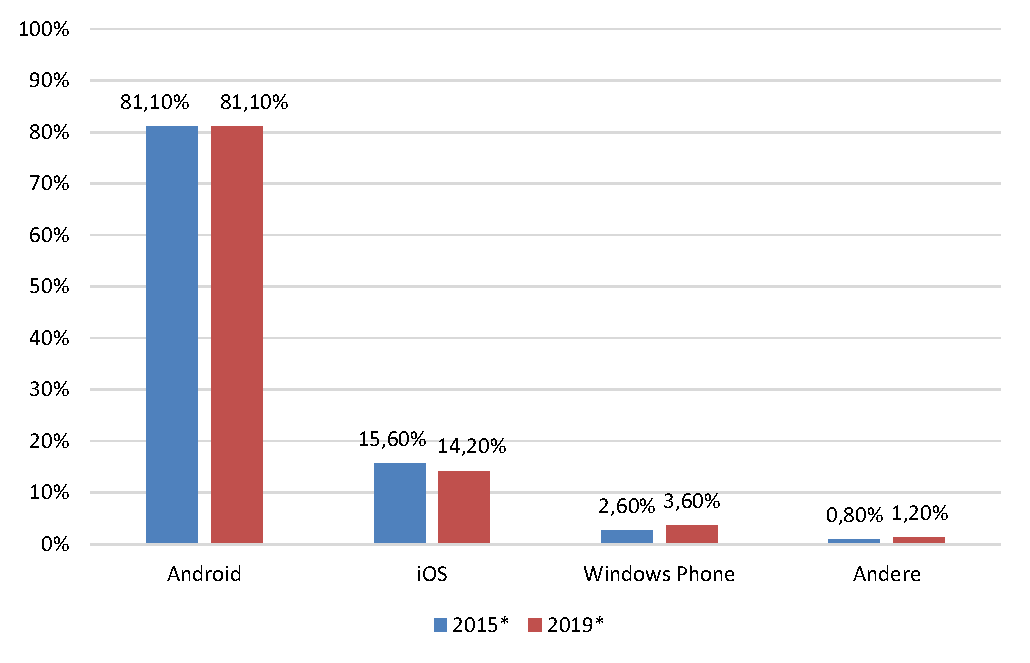
\includegraphics[width=0.8\textwidth]{Bilder/Marktanteile_Betriebssysteme}
	\caption{Prognose zu den Marktanteilen der Betriebssysteme am Absatz vom Smartphones weltweit in den Jahren 2015 und 2019}\label{graph_mobile_systems}\citep{marktanteile_betriebssysteme}
\end{figure}

Die Grafik verdeutlicht, dass aktuell Geräte mit Android Systemen den Markt eindeutig dominieren. Darauf folgen Geräte mit iOS und Windows Phone. Laut Prognose wird sich auch in den nächsten Jahren an dieser Hierarchie nichts ändern. Schlussfolgernd sind diese drei Systeme die relevantesten auf dem globalen Markt.

Abbildung \ref{graph_mobile_systems_laender} gibt Aufschluss über die Verteilung der Systeme nach ausgewählten Ländern. Die Daten beziehen sich auf die Verkäufe von August bis Oktober 2015, welche von Kantar im Dezember 2015 veröffentlicht wurden. Bei der Internationalisierung von Applikationen ist es von Vorteil zu wissen, wie stark die Gewichtung der Systeme in den einzelnen Ländern ist.

\begin{figure}[htbp]
	\centering
	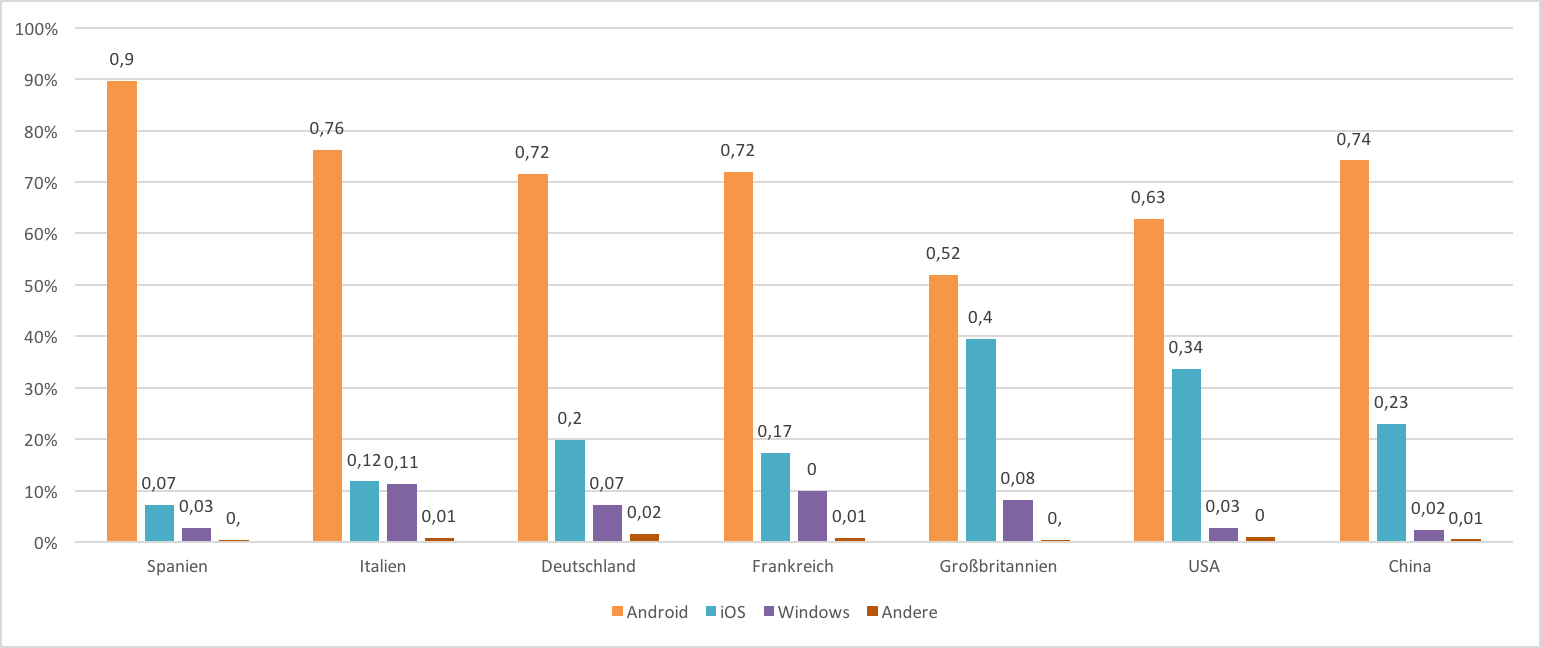
\includegraphics[width=0.8\textwidth]{Bilder/Marktanteile_nach_Laendern}
	\caption{Marktanteile der mobilen Betriebssysteme am Absatz von Smartphones in ausgewählten Ländern von August bis Oktober 2015}\label{graph_mobile_systems_laender}\citep{marktanteile_betriebssysteme_laender}
\end{figure}

\subsection{Verfügbare Applikationen und Kategorien der Stores}
Die Menge an verfügbaren Apps in den jeweiligen Stores ist unterschiedlich groß.
Eine Analyse über die aktiven Applikationen in den einzelnen Stores und die Gewichtung der Kategorien, soll einen Überblick verschaffen was die jeweiligen Plattformen aktuell zu bieten haben.
In Abbildung \ref{graph_apps_in_stores} wird die Menge an verfügbaren Apps im Mai 2015 dargestellt. Um eine bessere Übersicht zu gewährleisten, wurden die Werte gerundet. Der Amazon Appstore bietet wie der Google Play Store nur Android Apps an. Da es in diesen beiden Stores zum Teil zu Überschneidungen beim Angebot von Anwendungen kommt, werden diese Werte separat betrachtet und nicht summiert.

\begin{figure}[htbp]
	\centering
	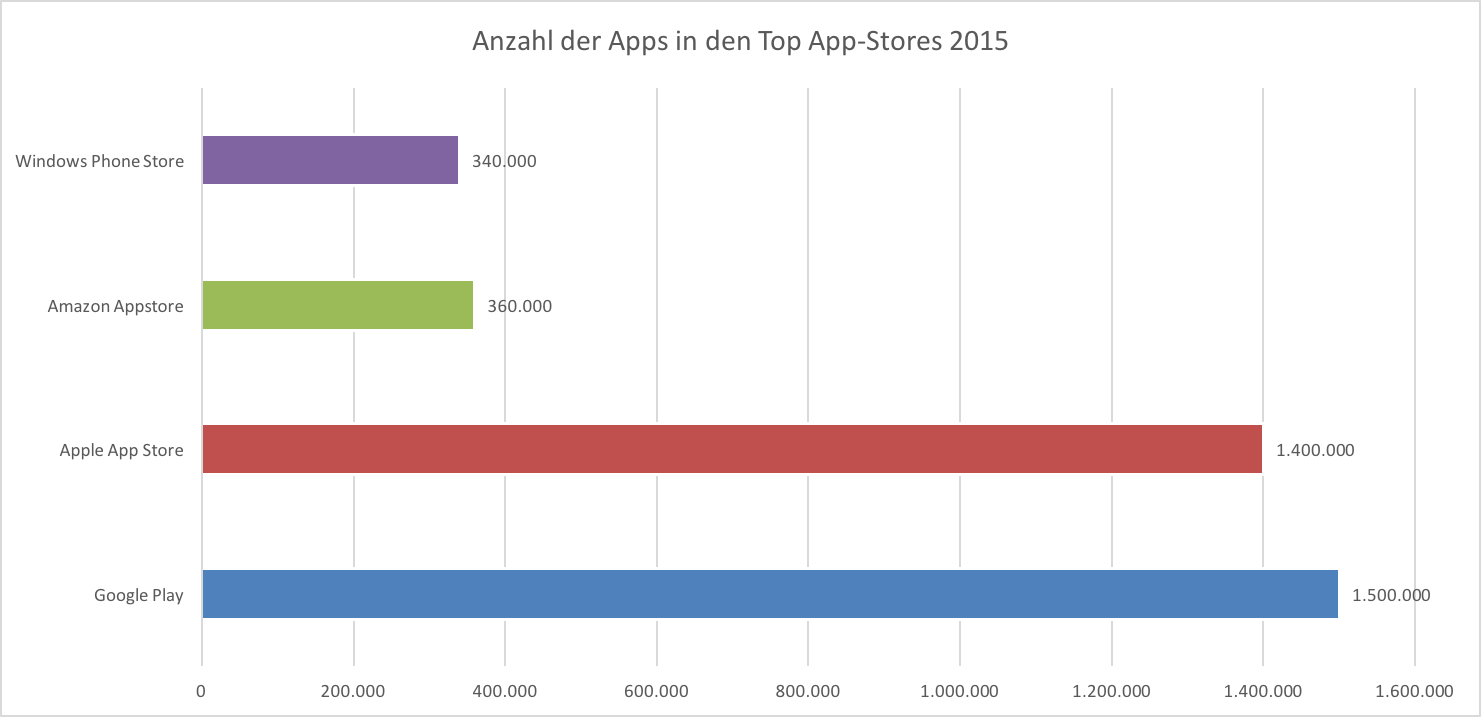
\includegraphics[width=0.8\textwidth]{Bilder/Anzahl_der_Apps}
	\caption{Anzahl der angebotenen Apps in den Top App-Stores im Mai 2015}\label{graph_apps_in_stores}\citep{apps_in_stores}
\end{figure}

Der Wert für den Windows Phone Store ist der Quelle nach von September 2014 und schließt damit noch nicht die Windows 10 Universal Apps mit ein. Diese kamen erst Mitte 2015 dazu und werden in einem getrenntem Windows Store hardwareübergreifend angeboten. Im September 2015 waren rund 80\% der Downloads aus dem Windows Phone Store von Geräten mit der Version 8.1, etwa 15\% von 8.0 Benutzern und etwa 5\% von der aussterbendem Version 7.8.
Laut Windows wurden im September 2015 etwa 50\% der Applikationen mit Windows 10 aus dem neuen Windows Store heruntergeladen. Diese Statistik gibt jedoch wenig Aufschluss wie groß dabei der Anteil an mobilen Systemen ist. Jedoch dominiert die Kategorie "Games" bei Windows 10 Apps mit fast 45\% die Downloadzahlen.\citep{windows_store_trends_2015}

\begin{figure}[htbp]
	\centering
	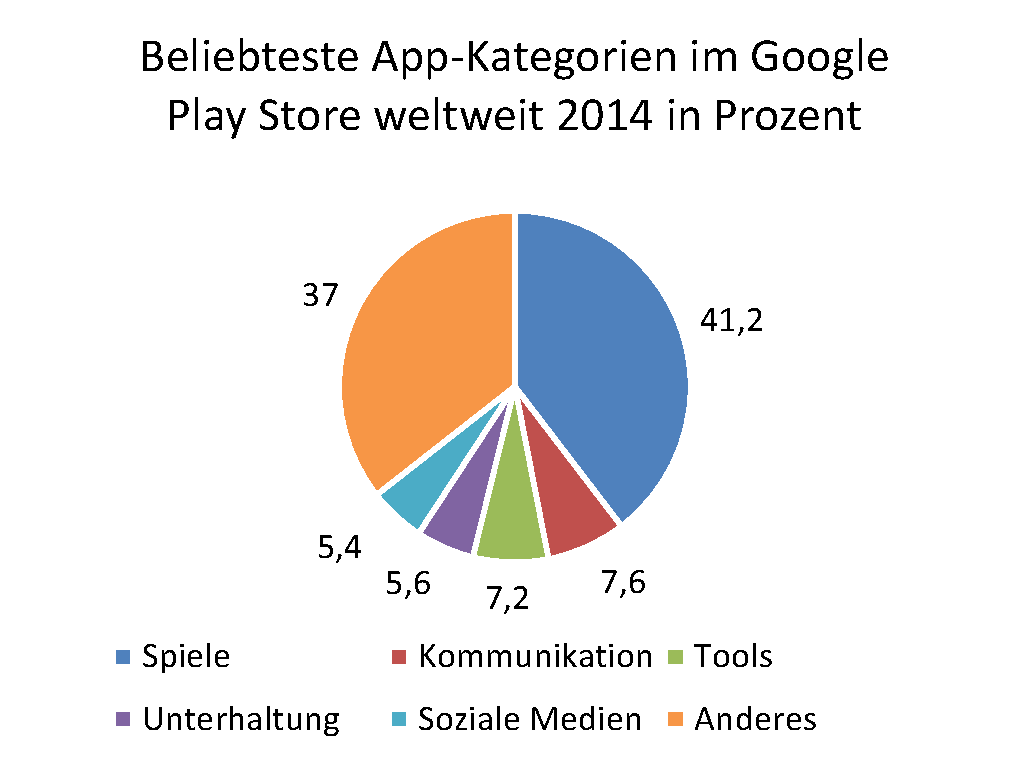
\includegraphics[width=0.8\textwidth]{Bilder/Google_Play_Store_Kategorien}
	\caption{Anteil der im Google Play Store weltweit am häufigsten heruntergeladenen Apps nach Kategorien im Februar 2014}\label{graph_play_store_kategorien}\citep{play_store_categories}
\end{figure}

Auch im Google Play Store werden Spiele Apps am häufigsten heruntergeladen und nehmen etwa 41\% des Downloadvolumens ein.(Abb.\ref{graph_play_store_kategorien})

\begin{figure}[htbp]
	\centering
	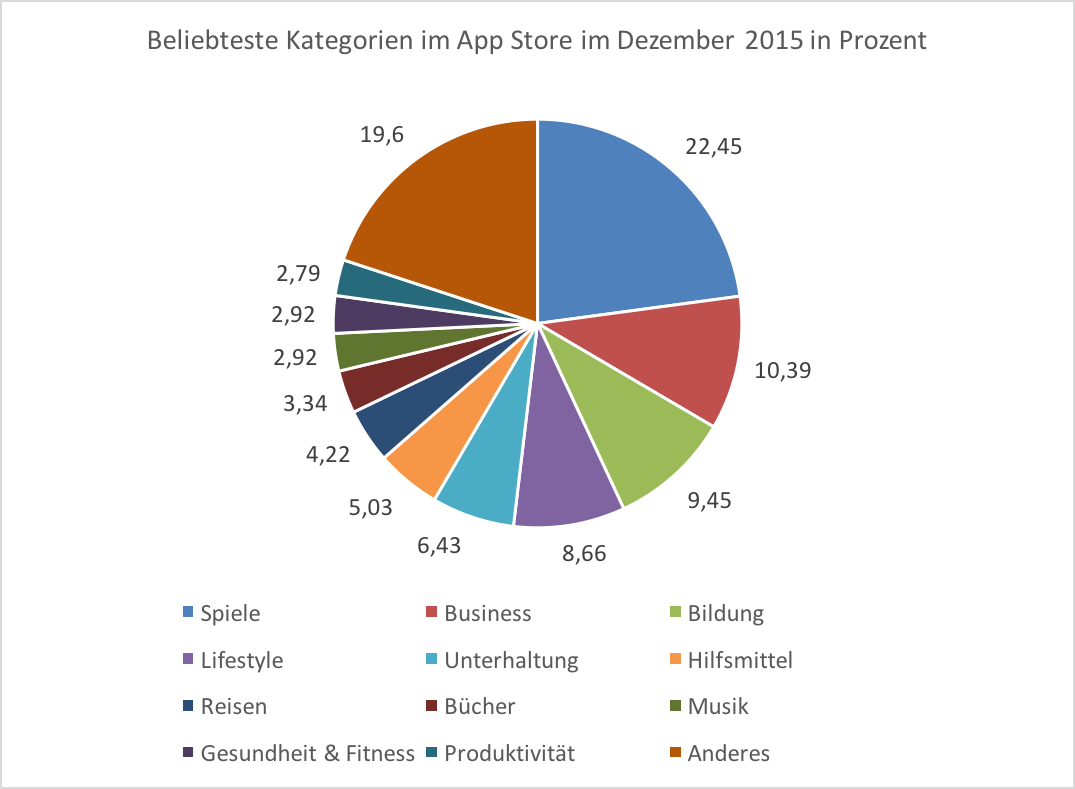
\includegraphics[width=0.8\textwidth]{Bilder/Top_Kategorien_App_Store}
	\caption{Ranking der Top-Kategorien im App Store im Dezember 2015}\label{graph_app_store_kategorien}\citep{app_store_categories}
\end{figure}

Die beliebtesten Kategorien des Apple App Store werden ebenfalls deutlich von den Spielen angeführt. Auch wenn der Abstand zur zweithäufigsten Kategorie geringer ist als bei den anderen Stores, macht der Spielebereich trotzdem etwa ein viertel aller Downloads aus.(Abb.\ref{graph_app_store_kategorien})
\medskip

Auch wenn jeder Store seine Applikationen auf eigene Weise kategorisiert, ist dennoch klar zu erkennen das Spiele bei jedem Anbieter das höchste Downloadvolumen ausmachen und sich stetig wachsender Beliebtheit erfreuen. Die Nachfrage nach mobilen Spielen ist demnach plattformübergreifend und berechtigt die Evaluierung von entsprechender Entwicklungssoftware.

\section{Betrachtung der mobilen Systeme}
Anhand der gewonnenen Erkenntnisse aus Kapitel \ref{subsec:Marktanteile_mobile_Systeme}, spielen derzeit die mobilen Systeme von Android, iOS und Windows Phone die größte Rolle auf dem Markt und bei den Benutzern. Folglich werden weitere Systeme nicht weiter betrachtet und der Fokus auf diese drei Systeme gerichtet.

\subsection{Android}
Android ist ein Open Source Betriebssystem und gleichzeitig eine Software-Plattform, welches stark im mobilen Bereich vertreten ist und auf dem Linux-Kernel basiert. Zu finden ist diese auf Smartphones, Tablet-Computern, Netbooks und auch auf Smart-TV Geräten. \citep{android_overview} Entwickelt wird Android von der Open Handset Alliance (OHA), welche von Google gegründet wurde. Die OHA wurde im November 2007 gegründet und ist ein Konsortium von mehr als 80 Unternehmen aus den Bereichen Mobilfunknetz, Geräteherstellung, Halbleiterindustrie, Marketing und Software. \citep{alliance_members} Der Grund für die Entwicklung von Android war und ist es, einen offenen Standard für mobile Geräte zu schaffen. \citep{alliance_overview}

Durch seine Offenheit ermöglicht Android Entwicklern große Freiheit bei der Programmierung von Applikationen. Eigene Entwicklungen können auch mit Anwendungen von Google, wie zum Beispiel Google Maps, verknüpft werden.

Auch der Hardwarebereich bietet ein breites Spektrum an Geräten mit kostengünstigen, bis hochpreisigen Angeboten, sowohl mit einfacher bis qualitativ hochwertiger, technischer Ausstattung. Benutzer haben die Möglichkeit, ihre Geräte weitestgehend frei zu gestalten und einzustellen. Für die Installation von neuen Applikationen sind diese auch nicht an einen einzigen Store gebunden und können Apps auch aus verschiedensten Quellen beziehen.
\\

Vorteile:
\begin{itemize}
	\item Open Source
	\item Unabhängigkeit von Anbietern
	\item Personalisierung
	\item Hardwareangebot
\end{itemize}

Nachteile:
\begin{itemize}
	\item Hohe Verbreitung von Schadsoftware
	\item Aktualität der Version ist abhängig vom Gerätehersteller
\end{itemize}

\subsection{iOS}
iOS ist das mobile Betriebssystem des Unternehmen Apple. Dieses ist ein Derivat von Mac OS X, welches selbst auf Unix basiert. Es wird ausschließlich von Apple entwickelt und ist somit nur auf den eigenen Geräten iPhone, iPad und iPod touch zu finden. Mit der Entwicklung wurde unter externer und interner Geheimhaltung 2005 begonnen und das Resultat der Öffentlichkeit zum ersten Mal Anfang 2007 vorgestellt. Bis zur Version 4.0 wurde iOS mit dem Namen iPhoneOS betitelt. Das Konzept und Design ist schwerpunktmäßig auf hohe Benutzerfreundlichkeit und Funktionalität ausgelegt. 

Durch die geschlossene Struktur des Systems sind eigene Derivate nicht möglich. Benutzer sind für den offiziellen Bezug von Applikationen auf Apples App Store angewiesen.
Bei der Wahl der Hardware ist man auf die Produktpalette von Apple angewiesen, welche jährlich eine neue Generation veröffentlicht. Die Personalisierung der Geräte ist nur bedingt möglich, da Anbieter von Drittsoftware keinen Zugriff auf das System haben und Anwendungen nur offiziell über den eigenen App Store bezogen werde können. Dies bietet jedoch den Vorteil einer Qualitätssicherung durch Apple, da Applikationen vor der Veröffentlichung einer Prüfung unterzogen werden.
\\

\textbf{Vorteile:}
\begin{itemize}
	\item Kompatibilität von Software und Hardware
	\item Benutzerfreundlichkeit
	\item Geräteübergreifende Kommunikation
	\item Kontrollen bei Veröffentlichung von Anwendungen
\end{itemize}

\textbf{Nachteile:}
\begin{itemize}
	\item Restriktive Firmenpolitik
	\item Proprietäres System
	\item Hardwareauswahl
	\item Anwendungen nur über den App Store
\end{itemize}

\subsection{Windows Phone}
Entwickler Microsoft stellt seit dem Jahr 2000 Betriebssysteme für mobile Geräte her. \citep{microsoft_mobile} 
Seitdem hat sich die Namensgebung von Windows Mobile, über Windows Phone, bis zum aktuellsten Windows 10 Mobile vorgearbeitet. Um im allgemeinen Bezug nicht zwischen den Namen hin und her zu wechseln, wird in dieser Arbeit, wenn mobile Windows Systeme erwähnt werden, der Name Windows Phone benutzt.
Die frühen Versionen von Windows Phone, also Windows Mobile und Windows Phone 7 stammen noch von dem Windows CE Kernel ab, wobei die aktuellen Versionen, Windows Phone 8 und Windows 10 Mobile, Derivate des Windows NT Kernels sind. Mit dem neuesten Ableger, Windows 10 Mobile, verspricht Microsoft eine homogene Kommunikations- und Anwendungsstruktur zwischen allen Geräten die mit diesem System betrieben werden. Dazu zählen nicht nur Smartphones und Tablets, sondern auch Notebooks, Desktop PCs und die Spielkonsole Xbox One. \citep{windows10_features}

Microsoft verfolgt mit Windows Phone eine ähnlich geschlossene und proprietäre Struktur wie der Konkurrent Apple. Eigene Derivate des Systems sind also nicht offiziell möglich. Auch die Benutzer müssen für neue Anwendungen auf das Angebot des Windows Stores zurückgreifen. Jedoch will Microsoft Entwicklern die Möglichkeit bieten, zukünftige Anwendungen universell verfügbar zu machen, das diese auf allen Windows Systemen nutzbar sind. Microsoft arbeitet außerdem an einer Technik, die bestehende Android und iOS Anwendungen auf die Windows Plattform überführen kann. \citep{wp_with_android_ios}

Die aktuellen Windows Phone Versionen sind durch eine Allianz von Windows und Nokia, hauptsächlich auf mobilen Geräten von Nokia zu finden.\citep{microsoft_nokia}
Aber auch andere Hersteller bieten Geräte mit Windows Phone, jedoch bisher in einem überschaubaren Umfang.
\\

Vorteile:
\begin{itemize}
	\item Kompatibilität von Software und Hardware
	\item Universelle Anwendungen
	\item Benutzerfreundlichkeit
\end{itemize}

Nachteile:
\begin{itemize}
	\item Proprietäres System
	\item Anwendungen nur aus dem Windows Store
	\item Geringeres Angebot an Anwendungen
\end{itemize}
\citep{wp_pros_cons}

%OPTIONAL!!!
%subsection{Weitere Systeme}

%TODO: Kapitel 3
\chapter{Native Softwareentwicklung}
Softwareentwicklung für ein bestimmtes System wird als nativ (lat.: angeboren, natürlich) bezeichnet. Hier sind Dateiformate, Programmiersprachen, Hardware, Entwicklungsumgebungen und Kompilierung genau an die Zielplattform angepasst. Nativer Code ist in der Lage alle individuellen Eigenschaften einer Zielplattform anzusprechen, ohne dabei eine eventuelle Portierbarkeit zu berücksichtigen.
\citep{native_software}
Welche Anforderungen iOS, Android und Windows Phone bezüglich nativer Entwicklung voraussetzen, soll in diesem Kapitel näher erläutert werden.

\section{Systemvorraussetzungen}
Um Applikationen für eine bestimmte Zielplattform zu entwickeln, werden unter Umständen Voraussetzungen an das Betriebssystem des Entwicklers gestellt.

\subsection{Android}
Die Entwicklung von Android Applikationen ist an kein bestimmtes System gebunden. Somit lassen sich diese unter Windows, OS X und Linux Systemen entwickeln. 
Windows Benutzer sollten mindestens Windows XP nutzen. Darüber hinaus können alle aktuelleren Versionen genutzt werden, wobei alle 32-Bit Editionen unterstützt werden und ab Windows 7 auch die mit 64-Bit.
Mac Systeme werden ab OS X 10.5.8 von den offiziellen Entwicklungswerkzeugen unterstützt.
Um auf einem Linux System zu entwickeln, kann man dies beispielsweise unter Ubuntu ab Version 8.04 tun. Bei 64-Bit Versionen ist es notwendig, dass diese fähig ist 32-Bit Anwendungen auszuführen. Da die Auswahl an Linux-Distributionen sehr umfangreich ist, wird an dieser Stelle auf diese nicht weiter eingegangen.
\citep{android_sdk_requirements}

\subsection{iOS}
%TODO

\subsection{Windows Phone}
%TODO

\section{SDKs und Versionen}
Software Development Kits, kurz SDKs, liefern dem Entwickler die Werkzeuge, Anwendungen und bestenfalls eine aktuelle Dokumentation, um für eine bestimmte Zielplattform zu entwickeln. Auch sind sie notwendig, um geschriebenen Code zu interpretieren und kompilieren. Um die aktuellste Version eines mobilen Systems zu unterstützen, muss das SDK auf ebenso aktuellen Stand sein.

\subsection{Android Versionen}
Android Versionen sind nach süßen Leckereien benannt und dem Anfangsbuchstaben nach alphabetisch aufsteigend. (Abb.\ref{tab_android_vers})

\begin{table}[htbp]
	\centering
	\resizebox{0.8\textwidth}{!}{%
		\begin{tabular}{|c|c|c|c|}
			\hline
			\rowcolor[HTML]{000000} 
			{\color[HTML]{FFFFFF} \textbf{Codename}} & {\color[HTML]{FFFFFF} \textbf{Version}} & {\color[HTML]{FFFFFF} \textbf{API Level}} & {\color[HTML]{FFFFFF} \textbf{Erscheinungsdatum}} \\ \hline
			Marshmallow                              & 6                                       & 23                                        & 5. Oktober 2015                                   \\ \hline
			Lollipop                                 & 5.1.x                                   & 22                                        & 9. März 2015                                      \\ \hline
			Lollipop                                 & 5.0.x                                   & 21                                        & 3. November 2014 - 19. Dezember 2014              \\ \hline
			Wear                                     & 4.4W                                    & 20                                        & Juni 2014                                         \\ \hline
			KitKat                                   & 4.4.x                                   & 19                                        & 31. Oktober 2013 - 19. Juni 2014                  \\ \hline
			Jelly Bean                               & 4.3.x                                   & 18                                        & 24. Juli 2013 - 4. Oktober 2013                   \\ \hline
			Jelly Bean                               & 4.2.x                                   & 17                                        & 13. November 2012 - 12. Februar 2013              \\ \hline
			Jelly Bean                               & 4.1.x                                   & 16                                        & 27. Juni 2012 - 10. Oktober 2012                  \\ \hline
			Ice Cream Sandwich                       & 4.0.3 - 4.0.4                           & 15, NDK 8                                 & 16. Dezember 2011 - 4. Februar 2012               \\ \hline
			Ice Cream Sandwich                       & 4.0 - 4.0.2                             & 14, NDK 7                                 & 19. Oktober 2011 - 15. Dezember 2011              \\ \hline
			Honeycomb                                & 3.2.x                                   & 13                                        & 16. Juli 2011                                     \\ \hline
			Honeycomb                                & 3.1                                     & 12, NDK 6                                 & 10. Mai 2011                                      \\ \hline
			Honeycomb                                & 3                                       & 11                                        & 23. Februar 2011                                  \\ \hline
			Gingerbread                              & 2.3.3 - 2.3.7                           & 10                                        & 23. Februar 2011 - 20. September 2011             \\ \hline
			Gingerbread                              & 2.3 - 2.3.2                             & 9, NDK 5                                  & 6. Dezember 2010 - Januar 2011                    \\ \hline
			Froyo                                    & 2.2 - 2.2.2                             & 8, NDK 4                                  & 20. Mai 2010 - Januar 2011                        \\ \hline
			Eclair                                   & 2,1                                     & 7, NDK 3                                  & 12. Dezember 2010                                 \\ \hline
			Eclair                                   & 2.0.1                                   & 6                                         & 3. Dezember 2009                                  \\ \hline
			Eclair                                   & 2                                       & 5                                         & 26. Oktober 2009                                  \\ \hline
			Donut                                    & 1.6                                     & 4, NDK 2                                  & 15. September 2009                                \\ \hline
			Cupcake                                  & 1.5                                     & 3, NDK 1                                  & 30. April 2009                                    \\ \hline
			ohne Codename                            & 1.1                                     & 2                                         & 10. Februar 2009                                  \\ \hline
			ohne Codename                            & 1                                       & 1                                         & 23. September 2008                                \\ \hline
		\end{tabular}
	}
	\caption{Android Versionen und ihr Erscheinungsdatum}\label{tab_android_vers}\citep{android_codenames,android_version_releases}
\end{table}

\subsection{iOS Versionen}
Apple nutzt für seine Produkte Codenamen, die keinem bestimmten Muster folgen. Verbrauchern sind diese meist unbekannt, da diese überwiegend intern genutzt werden. (Abb.\ref{tab_ios_vers})

\begin{table}[htbp]
	\centering
	\resizebox{0.5\textwidth}{!}{%
		\begin{tabular}{|c|c|c|}
			\hline
			\rowcolor[HTML]{000000} 
			{\color[HTML]{FFFFFF} \textbf{Codename}} & {\color[HTML]{FFFFFF} \textbf{Version}} & {\color[HTML]{FFFFFF} \textbf{Erscheinungsdatum}} \\ \hline
			Monarch                                  & 9.2 Beta                                & 3. November 2015                                  \\ \hline
			Monarch                                  & 9.1                                     & 21. Oktober 2015                                  \\ \hline
			Monarch                                  & 9.0.x                                   & 16. September 2015                                \\ \hline
			Copper                                   & 8.4.x                                   & 30. Juni 2015                                     \\ \hline
			Stowe                                    & 8.3                                     & 8. April 2015                                     \\ \hline
			OkemoZurs                                & 8.2                                     & 9. März 2015                                      \\ \hline
			OkemoTaos                                & 8.1.x                                   & 9. Dezember 2015                                  \\ \hline
			Okemo                                    & 8.0.x                                   & 17. September 2014                                \\ \hline
			Sochi                                    & 7.1.x                                   & 10. März 2014                                     \\ \hline
			Innsbruck                                & 7.0.x                                   & 18. September 2013                                \\ \hline
			Brighton                                 & 6.1.x                                   & 21. Februar 2013                                  \\ \hline
			Sundance                                 & 6.0.x                                   & 19. September 2012                                \\ \hline
			Hoodoo                                   & 5.1.x                                   & 7. März 2012                                      \\ \hline
			Telluride                                & 5.0.x                                   & 12. Oktober 2011                                  \\ \hline
			Durango                                  & 4.3.x                                   & 9. März 2011                                      \\ \hline
			Jasper                                   & 4.2.x                                   & 22. November 2010                                 \\ \hline
			Baker                                    & 4.1                                     & 8. September 2010                                 \\ \hline
			Apex                                     & 4.0.x                                   & 21. Juni 2010                                     \\ \hline
			Wildcat                                  & 3.2.x                                   & 3. April 2010                                     \\ \hline
			Northstar                                & 3.1.x                                   & 9. September 2009                                 \\ \hline
			Kirkwood                                 & 3.0.x                                   & 17. Juni 2009                                     \\ \hline
			Timberline                               & 2.2.x                                   & 21. November 2008                                 \\ \hline
			Sugarbowl                                & 2.1.x                                   & 9. September 2008                                 \\ \hline
			Big Bear                                 & 2.x                                     & 11. Juli 2008                                     \\ \hline
			Little Bear                              & 1.1.x                                   & 14. September 2007                                \\ \hline
			Alpine                                   & 1.0.x                                   & 29. Juni 2007                                     \\ \hline
		\end{tabular}
	}
\caption{iOS Versionen und ihr Erscheinungsdatum}\label{tab_ios_vers}\citep{ios_codenames}
\end{table}


\subsection{Windows Phone Versionen}
%TODO

\section{Programmiersprachen}
In der nativen Entwicklung werden für jede Zielplattform bestimmte Programmiersprachen unterstützt. 

\subsection{Android}
Android Applikationen werden in Java entwickelt. Demnach ist es notwendig vorab eine aktuelle Java Version (JDK) zu installieren. Diese wird von dem Unternehmen Oracle, mit der aktuellen Version 8 Update 66, vertrieben.
\citep{java_jdk}

\subsection{iOS}
%TODO

\subsection{Windows Phone}
%TODO

%OPTIONAL!!!
%\subsection{Popularität der Programmiersprachen}

\section{Entwicklungsumgebungen}
Für die Entwicklung werden jeweilig verschiedene IDEs (Integrated Development Environment) seitens der Betreiber unterstützt und empfohlen. Eine Besonderheit bei IDEs für mobile Systeme ist die Unterstützung eines Simulators. Dieser simuliert ein spezifiziertes Gerät auf virtuelle Weise, um Entwicklungen direkt testen zu können.

\subsection{Android}
Android empfiehlt das eigene Android Studio, welches die offizielle IDE für Android Entwicklung darstellt und zusätzlich das aktuelle SDK mitliefert. Android Studio basiert auf der IDE IntelliJ IDEA und ist frei verfügbar.\citep{android_studio} Alternativer Vorgänger ist die quelloffene IDE Eclipse.

\subsection{iOS}
%TODO

\subsection{Windows Phone}
%TODO

\section{Zusammengefasste Übersicht}
Die Tabelle \ref{platform_differnces} soll eine kompaktere Übersicht der einzelnen Systeme bieten.

\begin{table}[htbp]
	\centering
	\resizebox{\textwidth}{!}{%
		\begin{tabular}{c|c|c|c|c|c|c|c|c|}
			\cline{2-9}
			& \cellcolor[HTML]{036400}{\color[HTML]{FFFFFF} \textbf{Virtuelle Maschine}} & \cellcolor[HTML]{036400}{\color[HTML]{FFFFFF} \textbf{Programmiersprache}} & \cellcolor[HTML]{036400}{\color[HTML]{FFFFFF} \textbf{User Interface}} & \cellcolor[HTML]{036400}{\color[HTML]{FFFFFF} \textbf{Memory Management}} & \cellcolor[HTML]{036400}{\color[HTML]{FFFFFF} \textbf{IDE}} & \cellcolor[HTML]{036400}{\color[HTML]{FFFFFF} \textbf{Plattform}} & \cellcolor[HTML]{036400}{\color[HTML]{FFFFFF} \textbf{Geräte}} & \cellcolor[HTML]{036400}{\color[HTML]{FFFFFF} \textbf{App Markt}} \\ \hline
			\multicolumn{1}{|c|}{\cellcolor[HTML]{00009B}{\color[HTML]{FFFFFF} \textbf{Android}}}       & Dalvik VM                                                                  & Java                                                                       & XML files                                                              & Garbage collector                                                         & Eclipse, Android Studio                                                     & Multi-platform                                                    & Heterogen                                                      & Google Play Store                                                 \\ \hline
			\multicolumn{1}{|c|}{\cellcolor[HTML]{00009B}{\color[HTML]{FFFFFF} \textbf{iOS}}}           & -                                                                          & Objective-C, Swift                                                         & Cocoa Touch                                                            & Reference counting                                                        & XCode                                                       & Mac OS X                                                          & Homogen                                                        & Apple Apps Store                                                  \\ \hline
			\multicolumn{1}{|c|}{\cellcolor[HTML]{00009B}{\color[HTML]{FFFFFF} \textbf{Windows Phone}}} & CLR                                                                        & C\# and .Net                                                               & XAML files                                                             & Garbage collector                                                         & Visual Studio                                               & Windows                                                           & Homogen                                                        & Windows Phone Store                                               \\ \hline
		\end{tabular}
	}
	\caption{Unterschiede zwischen Android, iOS und Windows Phone}
	\label{platform_differnces}
\end{table}

%OPTIONAL!!!
%\section{Kompilierung}

%OPTIONAL!!!
%TODO: Kapitel 8
%\chapter{Stores für mobile Spiele}
%\section{Allgemeine Bedingungen für Entwickler}
%\section{Maximale App-Größe}
%\section{Anforderungen an den Quellcode}
%\section{Kosten und Abgaben}

%TODO: Kapitel 4
\chapter{Plattformübergreifende Entwicklung}
Die Entwicklung von Software-Produkten und Services, welche auf mehreren Systemen oder Laufzeitumgebungen funktioniert, wird als plattformübergreifende oder auch Cross-Plattform Entwicklung definiert. Um dies zu gewährleisten nutzen Entwickler unterschiedliche Methoden und Techniken, um verschiedene Systeme mit einer Projektstruktur zu erreichen.\citep{cross_plattform_explanation}

\begin{figure}[htbp]
	\centering
	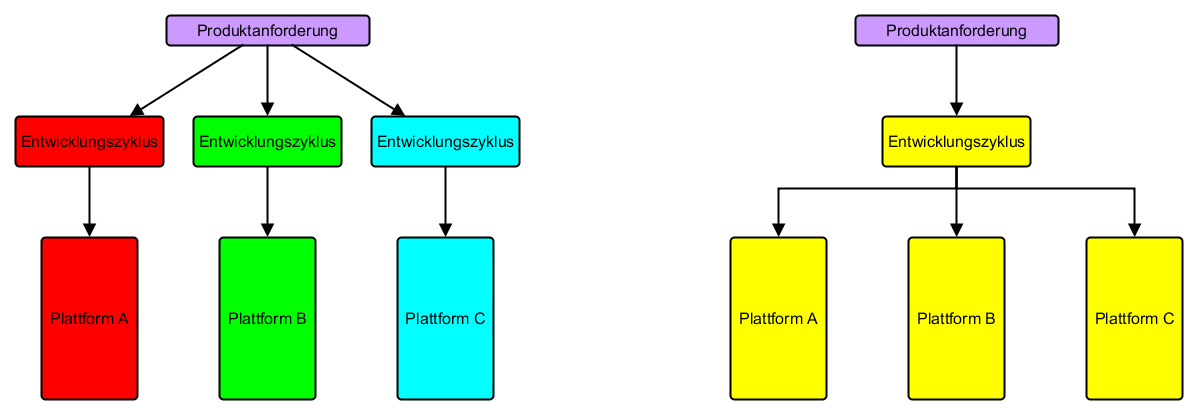
\includegraphics[width=0.8\textwidth]{Bilder/nativ_vs_cross}
	\caption{Traditionelle und plattformübergreifende Entwicklungsmodelle}\label{graph_nativ_vs_cross}
\end{figure}


\section{Ziel}
Die Idee und das Ziel von plattformübergreifender Entwicklung sind, dass eine Softwareanwendung auf mehr als einer spezifischen digitalen Umgebung zufriedenstellend funktioniert. Diese Vorgehensweise wird angewandt, um ein Softwareprodukt auf mehreren proprietären Betriebssystemen zu vertreiben. Dies soll die Entwicklungszeit und sich daraus ergebene Kosten einsparen. Durch die Entwicklung von mobilen Geräten, sowie die zunehmende Verbreitung von Open Source Technologien, entstanden sukzessiv unterschiedliche Ansätze zur Realisierung.

Die Nutzung dieser Arbeitsweisen hat aber nicht nur Vorteile. Als nachteilig gilt die potentiell geringere Effizienz der Anwendung gegenüber der nativen Entwicklung. Beispielsweise enthält es redundante Prozesse oder für jede Plattform einen eigenen Datenspeicherordner. Die Reduzierung von Komplexitäten kann auch bis zur „Verdummung“ ausarten, um das Programm für weniger anspruchsvolle Softwareumgebungen anzugleichen. 

Trotz mancher momentanen Grenzen bietet die plattformübergreifende Entwicklung ausreichende Möglichkeiten, die eine derartige Projektstruktur befürworten.\citep{cross_plattform_explanation}

\section{Funktionsweise und Realisierungsansätze}
Zu den grundlegenden Strategien gehört, dass ein Projekt oder Programm in verschiedene spezifische Betriebssystemversionen kompiliert wird. Weitere Methoden beinhalten die Verwendung von Teilbäumen in der Projektstruktur, um die Anwendung bestmöglich an die Eigenheiten der entsprechenden Zielplattform anzupassen. Ein anderer Ansatz ist die Abstraktion des Codes auf unterschiedlichen Ebenen, um sich mehreren Softwareumgebungen anzunähern. Softwareprojekte die diese Verfahren anwenden, kann man als plattformunabhängig, genauer gesagt plattformübergreifend bezeichnen, da sie die unterstützten Systeme gleich wertet und keines bevorzugt.\citep{cross_plattform_explanation}

\medskip
Die Entwicklung von plattformübergreifenden Anwendungen auf mobilen Systemen wird in sechs verschiedene Ansätze kategorisiert. (Abb.\ref{graph_cross_plattform_approaches})

\begin{figure}[htbp]
	\centering
	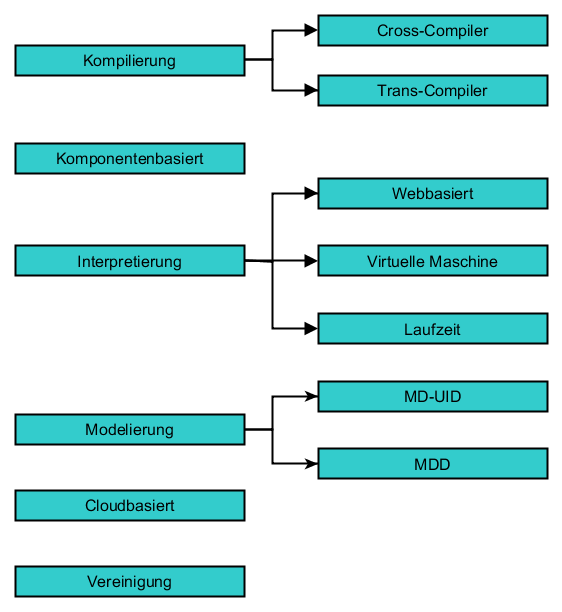
\includegraphics[width=0.5\textwidth]{Bilder/Cross_Plattform_Ansaetze}
	\caption{Haupt- und Nebenansätze zur Entwicklung von mobilen plattformübergreifenden Anwendungen}\label{graph_cross_plattform_approaches}
\end{figure}

In den folgenden Unterkapiteln werden die einzelnen Ansätze und Unteransätze näher betrachtet. Die Analyse und Betrachtung basiert auf den Informationen der Ausaurbeitung von \citep{cross_plattform_approaches}.

\subsection{Kompilierung}
Kompilierung(Compilation) ist ein Ansatz mit zwei Unterkategorien:

\begin{itemize}
	\item Cross-Compiler
	\item Trans-Compiler
\end{itemize}

Der Compiler ist ein Programm, welches den Quellcode einer High-Level Programmiersprache in einen Low-Level Code übersetzt wird. Dieser Low-Level Code ist ein Binärcode in Maschinensprache, der von dem Prozessor verstanden wird. Dieser Konvertierungsprozess wird als Kompilierung bezeichnet.

\medskip
Man spricht von einem \textbf{Cross-Compiler}, wenn das System des Compilers unterschiedlich zu dem System ist, auf dem der kompilierte Code läuft. Die Zielsysteme können Betriebssysteme, Prozessoren oder eine Kombination aus beiden sein. Abb. \ref{graph_compilation_XMLVM} stellt eine von XMLVM gebotene Lösung zu Cross-Compiling dar. Dies nutzt XML für die Frontend Darstellung und für die Verarbeitung des Bytecodes eine virtuelle Maschine(VM).

\begin{figure}[htbp]
	\centering
	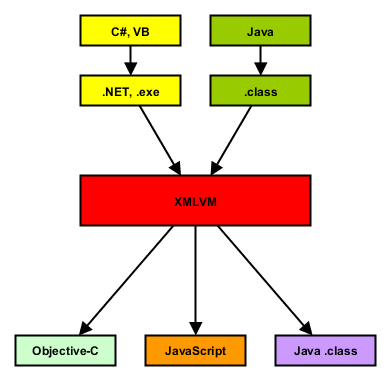
\includegraphics[width=0.5\textwidth]{Bilder/Compilation_Cross_XMLVM}
	\caption{XMLVM Prozess mit Java oder .NET Quellcode}\label{graph_compilation_XMLVM}\citep{XMLVM_Toolchain}
\end{figure}

\medskip
Ein \textbf{Trans-Compiler} kompiliert eine High-Level Programmiersprache in eine andere High-Level Programmiersprache. Da viele Sprachen jedoch unterschiedliche Eigenschaften und Leistungsmerkmale besitzen, muss der generierte Code unter Umständen nachbearbeitet werden, wenn der Compiler diese bei der Übersetzung nicht unterstützt. Auch ist der Code durch die automatisierte Erzeugung in der Regel nur schwer lesbar. Es besteht auch eine Abhängigkeit zu regelmäßigen Updates, um die Änderungen der Quell- und Zielsysteme aktuell zu halten.

%TODO
\subsection{Komponentenbasiert}
Die Komponente besteht aus einem Paket oder einem Modul, dessen Funktionen und Daten untereinander in Relation stehen. Jede Komponente besitzt eine Schnittstelle, dass die Servicedienste spezifiziert, welche von anderen Komponenten genutzt werden können. Die Kommunikation findet ausschließlich über die Schnittstellen statt, so dass eine Komponente keinerlei Informationen über den Aufbau einer anderen benötigt. 

\medskip
Ein beispielhafter Lösungsansatz ist der \textbf{Component-Based Mobile Web Application of Cross-Plattform}. Dieser komponentenbasierte Ansatz versucht die Entwicklung mobiler Web-Apps dahingehend zu vereinfachen, dass durch das Konzept von Softwarekomponenten, die Kernfunktionalitäten modular aufgeteilt werden. Diese Module beinhalten Speichermanagement, Netzwerkkommunikation, Grafik, Dateisystem und die Systemdienstkomponenten. Dadurch erhalten die Komponenten eine Wiederverwertbarkeit und vereinfacht die Migration auf andere Plattformen. Jede Plattform kann dieselben Schnittstellen nutzen, benötigt jedoch eine eigene innere Implementierung für die Unterstützung. 


\subsection{Interpretierung}
Bei der Interpretierung übersetzt ein Interpreter (Dolmetscher) den Quellcode in ausführbare Anweisungen. Dies geschieht in Echtzeit mit Hilfe einer dedizierten Maschine. Hierbei existieren drei Unteransätze:

\begin{itemize}
	\item Virtuelle Maschine (VM)
	\item Webbasiert (Web-based)
	\item Laufzeit Interpretation (Runtime Interpretation)
\end{itemize}

Die bekannteste \textbf{virtuelle Maschine} ist die Java Virtual Machine (JVM). Diese verfügt über eine eigene komplette Hardwarearchitektur wie einer CPU, Stack, Register und ein korrespondierendes Befehlssystem. Die Grundidee hierbei ist es die mobile App mit einer plattformübergreifenden Sprache zu entwickeln, die auf der dedizierten, virtuellen Maschine läuft und auf entsprechenden Plattformen installiert ist. In Abb. \ref{graph_interpreter_Dalvik} wird der Interpretierungsablauf der von Android bekannten Dalvik VM dargestellt.

\begin{figure}[htbp]
	\centering
	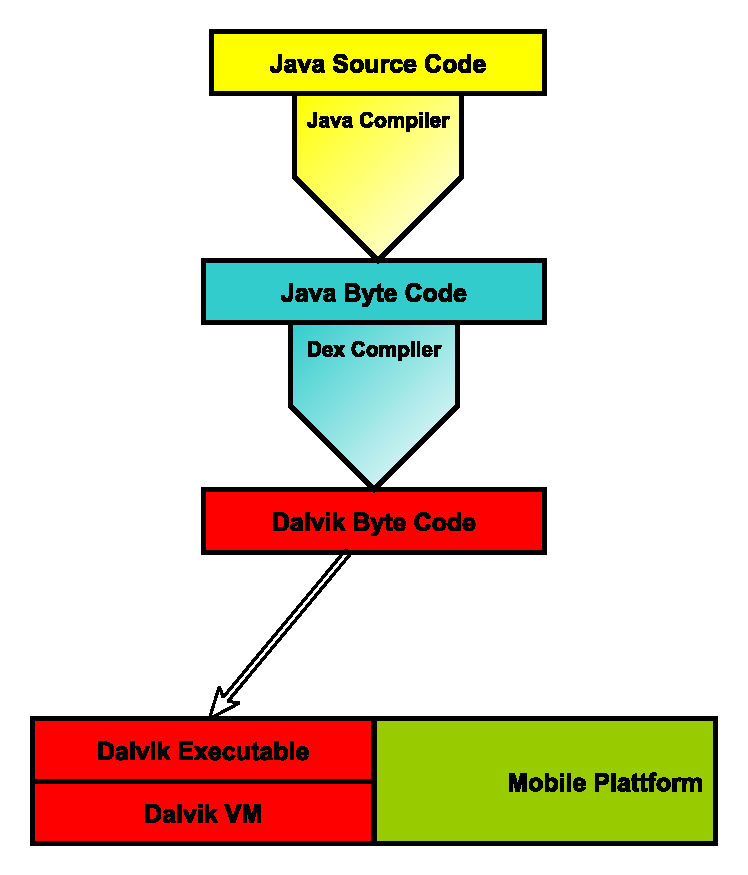
\includegraphics[width=0.5\textwidth]{Bilder/Interpretation_VM_Dalvik}
	\caption{Ablauf des Dalvik VM Interpreter}\label{graph_interpreter_Dalvik}
\end{figure}

\medskip
\textbf{Webbasierte} Tools verwenden Technologien wie HTML(5), Javascript und CSS, die auf verschiedenen Plattformen ausführbar sind. Der Zugriff auf Hardwarekomponenten wie Kamera und Sensoren erfolgt durch Wrapper. Wrapper sind Adapter oder Schnittstellen, um auf die nativen APIs zugreifen zu können. Abb. \ref{graph_interpreter_PhoneGap} zeigt die Kommunikation und Interpretierung des Webbasierten Interpreters PhoneGap von Adobe.

\begin{figure}[htbp]
	\centering
	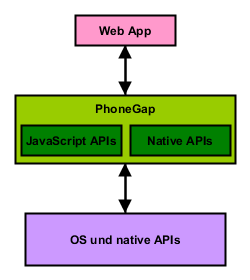
\includegraphics[width=0.3\textwidth]{Bilder/Interpretation_Web_PhoneGap}
	\caption{Vereinfachter Ablauf des PhoneGap Interpreters von Adobe}\label{graph_interpreter_PhoneGap}
\end{figure} 

\medskip
Die \textbf{Laufzeit} ist eine Ausführungsumgebung und eine Schicht, welche die mobile App auf der nativen Plattform lauffähig macht. Bei diesem Ansatz wird der Quellcode in Bytecode umgewandelt und dann zur Laufzeit von einer virtuellen Maschine ausgeführt. In Abb. \ref{graph_interpreter_Titanium} wird die Verarbeitung von Appcelerators Titanium-Interpreters dargestellt.

\begin{figure}[htbp]
	\centering
	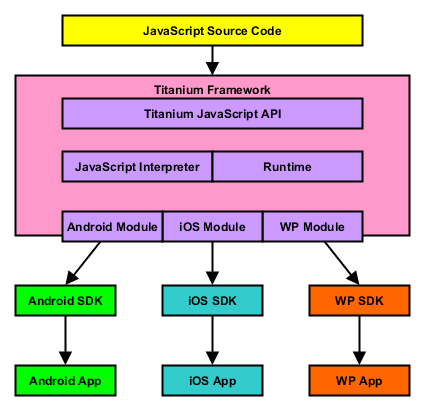
\includegraphics[width=0.5\textwidth]{Bilder/Interpretation_Runtime_Titanium}
	\caption{Ablauf des Titanium Interpreters von Appcelerator}\label{graph_interpreter_Titanium}
\end{figure}

\subsection{Modellierung}
Bei der Modellierung verwenden Entwickler abstrakte Modelle, um die Funktionen und / oder die Benutzeroberfläche der Anwendungen zu beschreiben. Diese Modelle werden für jede Zielplattform in entsprechenden Quellcode transformiert. Hierbei gibt es die Ansätze des Model-Based User Interface Development (MB-UID) und des Model-Driven Development (MDD).

\medskip
\textbf{MB-UID} wird genutzt, um die Benutzeroberfläche durch die formale Beschreibung von Aufgaben, Daten und Benutzern einer App automatisch zu generieren. Hierbei wird zwischen der Benutzeroberfläche und der App-Logik unterschieden.
Für die Generierung existieren zwei Strategien.

\begin{itemize}
	\item Eine Generierung zur Laufzeit der App, die eine Websysteme adaptiert und basiert auf Anfrage- und Antwortprotokollen (request / response). Eingeschränkt wird dies durch die Voraussetzung einer dauerhaften Verbindung zu einem Server.
	
	\item Die Generierung während der Entwicklungszeit, also vor Ausführung der Anwendung. Hier kann der Entwickler das generierte Interface überprüfen und zu jeder Plattform spezifische Funktionalitäten hinzufügen. Dabei kann die Funktion zur Verbindungsart festgelegt werden, also ob eine dauerhafte Verbindung bestehen soll oder zu einem selbst bestimmten Zeitpunkt synchronisiert werden soll.
\end{itemize}

\medskip
Das Hauptkonzept von \textbf{MDD} ist die Generierung von plattformspezifischen Versionen, basierend auf dem plattformunabhängigen, abstrakten Modell. Das Modell wird zum Beispiel durch Domain-Specific Language (DSL) beschrieben.

\subsection{Cloudbasiert}
In diesem Ansatz geschieht die Verarbeitung der Anwendung nicht lokal auf dem Gerät, sondern auf einem Cloudserver. Dabei werden einige Cloudeigenschaften verwendet, wie Flexibilität, Virtualisierung, Sicherheit und dynamisches Management. Die Clientanwendung ist dabei weitest möglich reduziert, da diese nur Basisprozesse benötigt. Dies wird Thin-Client genannt, da wie in Abb. \ref{client_aufgaben} nur Ein- und Ausgabe verarbeitet werden müssen. Cloudbasierte Anwendungen sollen dadurch besonders energieeffizient sein.

\begin{figure}[htbp]
	\centering
	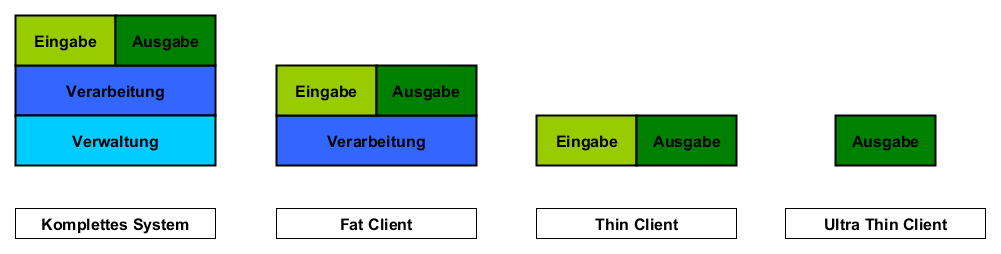
\includegraphics[width=0.8\textwidth]{Bilder/Aufgaben_Endgeraet}
	\caption{Aufgaben von Client-Anwendungen}\label{client_aufgaben}
\end{figure}

Da zur Zeit der Bearbeitung zu diesem Ansatz keine direkten Realisierungen gefunden worden, sondern überwiegend der theoretische Aufbau einer solchen Applikation, wird dieser Teil nicht weiter vertieft.

%TODO
\subsection{Vereinigung}
Dieser Ansatz versucht die besten Eigenschaften verschiedener Ansätze zusammenzuführen, von den jeweiligen Vorteilen zu profitieren und Nachteile zu minimieren.

\medskip
Ein \textbf{unbetitelter Lösungsansatz} vereinigt den komponentenbasierten Ansatz mit dem Cross Compiler und einer darauf angepassten Universalsprache. Um die nativen Hardwarefunktionen wie Kamera und GPS, sowie native Softwareeigenschaften wie Buttons und andere Interaktionsfelder anzusprechen, wird eine Sammlung an Komponenten erstellt. Implementierungen dieser Komponenten können durch gemeinsame Schnittstellen für jede Zielplattform erfolgen. Dieses Framework soll dem Entwickler ermöglichen, Applikationen zu entwickeln, die auf nativen Code und der Universalsprache basieren. Diese Sprache wird der App als zusätzliche Kommunikationsschicht und Schnittstelle hinzugefügt, um die Komponenten und deren Methoden anzusprechen.(Abb. \ref{graph_merge_component_based}) Der Entwickler implementiert nur eine minimale Struktur der App auf nativer Basis, welche die Benutzerschnittstelle und Navigation beinhaltet. An welcher Stelle und auf welche Weise die Komponenten integriert werden, wird durch die Universalsprache definiert. Das Framework regelt die Codeintegrierung innerhalb des nativen Codes. Bei diesem Lösungsansatz ist es erforderlich die Benutzerschnittstelle für jede Plattform manuell zu definieren. Dabei liegt der funktionale Fokus auf allgemeingültigen Funktionen, ohne Berücksichtigung der plattformspezifischen.

\begin{figure}[htbp]
	\centering
	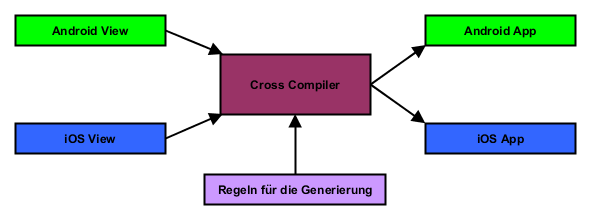
\includegraphics[width=0.8\textwidth]{Bilder/Merge_Component_based}
	\caption{Funktion eines komponentenbasierten Mergeansatz}\label{graph_merge_component_based}
\end{figure}

\medskip
\textbf{Integrated Cross-Platform Mobile Development (ICPMD)} ist eine weitere Lösung die auf dem Merge-Prinzip aufbaut und drei Verwendungsszenarios unterstützt. Diese Szenarios sind, wie in Abb. \ref{graph_merge_integrated_based} dargestellt, abhängig von dem gegebenen Input. 
Der Entwickler hat…
 
\begin{enumerate}
	\item …bereits ein bestehendes Projekt (z.B. Windows Phone) und möchte dies auf weitere Plattformen (z.B. iOS und Android) ausweiten.
	
	\item …definierte Anforderungen und möchte daraus, auf bestimmte Zielplattformen, eine mobile App erzeugen.
	
	\item …ein Projekt basierend auf dem abstrakten Modell und möchte dies aktualisieren und dann speichern oder daraus, auf bestimmte Zielplattformen, eine mobile App erzeugen.
\end{enumerate}

\begin{figure}[htbp]
	\centering
	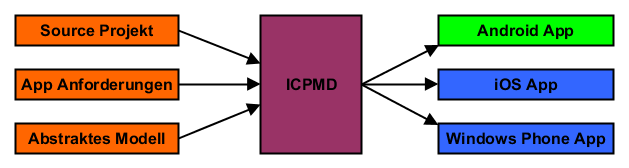
\includegraphics[width=0.8\textwidth]{Bilder/Merge_Integrated_based}
	\caption{Drei Szenarien bei ICPMD}\label{graph_merge_integrated_based}
\end{figure}

\section{Übersicht der Ansätze}
Tabelle \ref{table_all_approaches} fasst die vorigen Ansätze zur plattformübergreifenden Entwicklung in Kurzform zusammen, benennt die jeweiligen Vor- und Nachteile, sowie die Namen bekannter Lösungen.

\begin{table}[htbp]
	\centering
	\resizebox{0.8\textwidth}{!}{%
		\begin{tabular}{|c|c|p{5cm}|p{5cm}|p{1cm}|}
			\hline
			\rowcolor[HTML]{000000} 
			{\color[HTML]{FFFFFF} \textbf{Ansatz}} & {\color[HTML]{FFFFFF} \textbf{Unteransatz}} & \multicolumn{1}{c|}{\cellcolor[HTML]{000000}{\color[HTML]{FFFFFF} \textbf{Pro}}}                                                                                                                                                                                                                                                 & \multicolumn{1}{c|}{\cellcolor[HTML]{000000}{\color[HTML]{FFFFFF} \textbf{Contra}}}                                                                                                                    & \multicolumn{1}{c|}{\cellcolor[HTML]{000000}{\color[HTML]{FFFFFF} \textbf{\begin{tabular}[c]{@{}c@{}}Beispielhafte\\ Lösungsansätze\end{tabular}}}} \\ \hline
			\textbf{Kompilierung}                  & Cross-Compiler                              & Wiederverwertung eines existierenden Quellcodes durch Cross-Kompilierung auf eine andere Plattform.Die resultierende Applikation ist native und besitzt somit die Vorteile einer nativen App.                                                                                                                                    & Die Zuordnungen zwischen zwei Sprachen ist sehr aufwendig, so dass hauptsächlich die gemeinsamen Eigenschaften berücksichtigt werden.                                                                  & \begin{tabular}[c]{@{}l@{}}MoSync\\ Corona\\ Neomades\\ XMLVM\end{tabular}                                                                              \\ \hline
			\textbf{}                              & Trans-Compiler                              & Kann genutzt werden, um veraltete Applikationen und deren veralteter Code auf eine neuere Version derselben Sprache zu übersetzen. Wiederverwertung eines existierenden Quellcodes durch Trans-Kompilierung auf eine andere Plattform.Die resultierende Applikation ist native und besitzt somit die Vorteile einer nativen App. & Konzentriert sich ausschließlich auf die gemeinsamen APIs der Quell- und der Zielsprache. Benötigt regelmäßige Aktualisierungen, um die Änderungen der APIs in Quell- und Zielsprache zu unterstützen. & \begin{tabular}[c]{@{}l@{}}J2ObjC \\JUniversal\end{tabular}                                                                                                                                    \\ \hline
			\textbf{Komponentenbasiert}            &                                             & Vereinfacht die Unterstützung neuer Plattformen durch definierte Schnittstellen bei implementierten Komponenten.                                                                                                                                                                                                                 & Konzentriert sich nur auf die Gemeinsamkeiten der unterstützten Plattformen.                                                                                                                           & Theoretisch                                                                                                                                         \\ \hline
			\textbf{Interpretation}                & Webbasiert                                  & Leicht zu erlernen und zu benutzen, da es auf bekannten Web-Technologien aufbaut.                                                                                                                                                                                                                                                & Die Benutzerschnittstelle von webbasierten Apps besitzen nicht das gleiche Aussehen und Handhabung wie bei nativen Apps. Geringere Perfomance gegenüber nativen Apps.                                  & \begin{tabular}[c]{@{}l@{}} PhoneGap\\ Rhomobile\\xFace \end{tabular}                                           \\ \hline
			\textbf{}                              & Virtuelle Maschine                          & Geringere Gesamtgröße und schnellerer Download der Apps, da alle benötigten Bibliotheken und Funktionen in der VM gespeichert sind.                                                                                                                                                                                              & Langsame Ausführung der Applikation auf der VM. Die VM muss erst aus einem Store geladen werden, was auf iOS nicht unterstützt wird.                                                                   & MobDSL                                                                                                                                              \\ \hline
			\textbf{}                              & Laufzeit                                    & Der Quellcode muss nur einmal geschrieben werden.                                                                                                                                                                                                                                                                                & Die Perfomance beim Laden der App ist gering, da der Interpretierungsvorgang bei jeder einzelnen Ausführung stattfindet.                                                                               & \begin{tabular}[c]{@{}l@{}} Titanium\\ Xamarin \end{tabular}                                          \\ \hline
			\textbf{Modellierung}                  & MD-UID                                      & Spart Entwicklungszeit durch Generierung des UI-Codes. Nützlich für Prototyping, durch schnelle UI-Entwicklung und dadurch frühe Evaluierung der Benutzerfreundlichkeit.                                                                                                                                                         & Muss sich bei den einzelnen Plattformen auf ähnliche Benutzerschnittstellen konzentrieren.                                                                                                             & XMobile                                                                                                                                             \\ \hline
			\textbf{}                              & MDD                                         & Die Modellierungssprache ist effektiv, um Anforderungen zu definieren. Der Fokus liegt auf der Funktionalität und nicht an der technischen Implementierung.                                                                                                                                                                      & Kann existierenden, nativen Quellcode nicht verarbeiten.                                                                                                                                               & \begin{tabular}[c]{@{}l@{}}JSAF \\ MD2 \\ Jelly \\ AppliDE\end{tabular}                                                                             \\ \hline
			\textbf{Cloudbasiert}                 &                                             & Verarbeitungsprozesse werden in eine Cloud ausgelagert.                                                                                                                                                                                                                                                                          & Das Endgerät und die App benötigen eine schnelle, permanente Netzwerkverbindung.                                                                                                                       & Theoretisch                                                                                                                                         \\ \hline
			\textbf{Vereinigung}                   &                                             & Vorteile aus den Stärken anderer Ansätze. Bietet dem Entwickler vielseitige Möglichkeiten.                                                                                                                                                                                                                                       & Benötigt hohen Entwicklungsaufwand.                                                                                                                                                                    & ICPMD                                                                                                                                               \\ \hline
		\end{tabular}
	}
	\caption{Übersicht aller Ansätze}
	\label{table_all_approaches}
\end{table}

\section{Entwicklung mobiler Applikationen ohne den Schwerpunkt Spieleentwicklung}
In der Thesis „\textit{Plattformabhängige und –unabhängige Entwicklung mobiler Anwendungen am Beispiel von Geo-Wikipedia-App}“ \citep{cross_plattform_development_vehse} wird ebenfalls die plattformübergreifende Entwicklung analysiert, jedoch liegt hier nicht der Fokus auf Game-spezifischen Applikationen und Entwicklungswerkzeugen. Hier wird in Kapitel 2.2 auch auf die verschiedenen Herangehensweisen eingegangen und deren Resultate klassifiziert. Weiterhin wird eine Auswahl der bekannteren Cross-Plattform Entwicklungstools (PhoneGap, Xamarin, Appcelerator) analysiert. Diese Arbeit setzt den Schwerpunkt auf Frameworks und Engines zur Spieleentwicklung und geht von daher nicht weiter auf die genannten und vorangegangenen Entwicklungswerkzeuge ein.

%TODO: Kapitel 5
\chapter{Plattformübergreifende Frameworks zur Spieleentwicklung}
\section{Gamespezifische Frameworks und Engines}
\subsection{Cocos2D}
\subsection{Libgdx}
\subsection{Unity}
\subsection{Weitere Frameworks}
\section{Entwicklungsumgebungen}
\subsection{Unterstützte IDEs}
\subsection{Systembedingte Einschränkungen}

%TODO: Kapitel 6
\chapter{Gegenüberstellung der Frameworks}
%Features und Einschränkungen
\section{Zielplattformen}
%\section{Skalierbarkeit der Menge der Plattformen} % ???
\section{Programmiersprachen}
\section{Unterstützung von 2D und 3D}
\section{Zugriff auf Hardware}%Accelerometer etc
\section{Free- und Pro- Versionen}
\section{Einfluss auf Einstellungen}
\section{Zusätzlich benötigte Software}
\section{Aktualität - Versionen - Community}
\section{Zukunftsaussichten}

%OPTIONAL!!!
%TODO: Kapitel 7
%\chapter{Analyse der Marktanteile}
%\section{Menge an Firmen und Entwicklern}
%\section{Menge an Games}

%TODO: Kapitel 9
\chapter{Kosten-Nutzen Vergleich}
%Vergleichstabelle zu den Variationen der Projektanforderungen im Zusammenhang mit den Möglichkeiten und Kosten der Frameworks

%OPTIONAL!!!
%TODO: Kapitel 10
%\chapter{Grundgerüst und Aufbau eines Cross-Plattform Projekts}
%\section{Geteilter Content}
%\section{Plattformabhängiger Content}
%\section{Grundaufbau bei Engines}
%\section{Grundaufbau bei Frameworks}

%OPTIONAL!!!
%TODO: Kapitel 11
%\chapter{Game-typische Design Patterns und Architekturen}
%\section{Architekturen}
%\section{Patterns}
%\section{Verweis auf Bachelorarbeit: „Use of Design Patterns for mobile game Development“}

%OPTIONAL!!!
%TODO: Kapitel 12
%\chapter{Nutzen von Architekturen}
%\section{Pro}
%\subsection{Skalierbarkeit}
%\subsection{Lesbarkeit}
%\subsection{Wiederverwertbarkeit}
%\section{Contra}
%\subsection{KISS - Keep it simple stupid}

%TODO: Kapitel 13
\chapter{Konzeption und Implementierung einer Test-Applikation}
\section{Ideen}
\section{Anforderungen}
\section{Verwendete Frameworks und Engines}
\section{Verwendete APIs und SDKs}
\section{Assets und deren Verwendung}
%\section{User Stories}

%TODO
\chapter{Analyse messbarer Metriken}
%Kosten, Performance, Akkuverbrauch, App-Daten-Aufteilung, Größe des benötigten Speichers, Größe des geteilten Contents, Stabilität, RAM, Code-Zeilen/-Größe, Entwicklungszeit(bedingt zu berücksichtigen)

\chapter{Vergleich der Messprotokolle}

\chapter{Fazit}



%--------------------- VERZEICHNISSE -------------------------------------

\listoffigures % Abbildungsverzeichnis erzeugen
\listoftables % Tabellenverzeichnis erzeugen

%------------------------------ LITERATURVERZEICHNIS----------------------
%TODO:Alphabetisch sortieren!
%BIBTEX!?
\begin{thebibliography}{}

\bibitem[Open Handset Alliance - Android Overview(2015)]{android_overview}
\emph{Overview of Android by the Open Handset Alliance},
\url{http://www.openhandsetalliance.com/android_overview.html}, letzter Zugriff: 24.11.2015

\bibitem[Open Handset Alliance - Alliance Overview(2015)]{alliance_overview}
\emph{Overview of the Open Handset Alliance},
\url{http://www.openhandsetalliance.com/oha_overview.html}, letzter Zugriff: 24.11.2015

\bibitem[Open Handset Alliance - Alliance Members(2015)]{alliance_members}
\emph{Members of the Open Handset Alliance},
\url{http://www.openhandsetalliance.com/oha_members.html}, letzter Zugriff: 24.11.2015

\bibitem[Android Source - Codenames, Tags, and Build Numbers(2015)]{android_codenames}
\emph{Codenames, Tags, and Build Numbers in the history of Android},
\url{https://source.android.com/source/build-numbers.html}, etzter Zugriff: 24.11.2015

\bibitem[Wikipedia - Liste von Android-Versionen(2015)]{android_version_releases}
\emph{Übersicht von allen Android Versionen mit Veröffentlichungsdatum},
\url{https://de.wikipedia.org/wiki/Liste_von_Android-Versionen}, letzter Zugriff: 24.11.2015

\bibitem[John Daintith(2004)]{native_software}
\emph{A Dictionary of Computing - native software},
\url{http://www.encyclopedia.com/doc/1O11-nativesoftware.html}, letzter Zugriff: 24.11.2015

\bibitem[Sue Smith(2013)]{android_sdk_requirements}
\emph{Android SDK Requirements},
\url{http://code.tutsplus.com/tutorials/android-sdk-requirements--mobile-20086}, letzter Zugriff: 24.11.2015

\bibitem[the iphone wiki(2015)]{ios_codenames}
\emph{iOS Firmwares},
\url{https://www.theiphonewiki.com/wiki/Firmware}, letzter Zugriff: 24.11.2015

\bibitem[Oracle - Java SE(2015)]{java_jdk}
\emph{Java SE Development Kit 8 Downloads},
\url{http://www.oracle.com/technetwork/java/javase/downloads/jdk8-downloads-2133151.html}, letzter Zugriff: 24.11.2015

\bibitem[Android Develop Tools(2015)]{android_studio}
\emph{Android Studio Overview},
\url{http://developer.android.com/tools/studio/index.html}, letzter Zugriff: 24.11.2015

\bibitem[Reddit(2015)]{wp_pros_cons}
\emph{Reddit - Pros and cons of Windows phone, and why should I buy one instead of an android or a iPhone?},
\url{https://www.reddit.com/r/windowsphone/comments/3h21lf/pros_and_cons_of_windows_phone_and_why_should_i/}, letzter Zugriff: 25.11.2015

\bibitem[Microsoft(2014)]{microsoft_nokia}
\emph{Microsoft - Microsoft und Nokia Geräte},
\url{https://www.microsoft.com/de-de/nokia.aspx}, letzter Zugriff: 25.11.2015

\bibitem[Golem(2015)]{wp_with_android_ios}
\emph{Microsoft demonstriert Android- und iOS-Apps unter Windows},
\url{http://www.golem.de/news/windows-10-microsoft-demonstriert-android-und-ios-apps-unter-windows-1504-113812.html}, letzter Zugriff: 25.11.2015

\bibitem[Microsoft(2015)]{windows10_features}
\emph{Microsoft - Windows 10 Features},
\url{https://www.microsoft.com/de-de/windows/features}, letzter Zugriff: 25.11.2015

\bibitem[Fran Berkman(2012)]{microsoft_mobile}
\emph{Microsoft Mobile: From Pocket PC to Windows Phone 8},
\url{http://mashable.com/2012/10/29/microsoft-mobile-history/#DYxZxZ7wTuqD}, letzter Zugriff: 25.11.2015

\bibitem[IDC (2015)]{marktanteile_betriebssysteme}
\emph{Prognose zu den Marktanteilen der Betriebssysteme am Absatz vom Smartphones weltweit in den Jahren 2015 und 2019. In Statista - Das Statistik-Portal.},
\url{http://de.statista.com/statistik/daten/studie/182363/umfrage/prognostizierte-marktanteile-bei-smartphone-betriebssystemen/}, letzter Zugriff: 14.12.2015

\bibitem[Kantar (2015)]{marktanteile_betriebssysteme_laender}
\emph{Marktanteile der mobilen Betriebssysteme am Absatz von Smartphones in ausgewählten Ländern von August bis Oktober 2015. In Statista - Das Statistik-Portal.},
\url{http://de.statista.com/statistik/daten/studie/198453/umfrage/marktanteile-der-smartphone-betriebssysteme-am-absatz-in-ausgewaehlten-laendern/}, letzter Zugriff: 14.12.2015

\bibitem[Statista (2015)]{apps_in_stores}
\emph{Anzahl der angebotenen Apps in den Top App-Stores im Mai 2015. In Statista - Das Statistik-Portal.},
\url{http://de.statista.com/statistik/daten/studie/208599/umfrage/anzahl-der-apps-in-den-top-app-stores/}, letzter Zugriff: 14.12.2015

\bibitem[Distimo (2014)]{play_store_categories}
\emph{Anteil der im Google Play Store weltweit am häufigsten heruntergeladenen Apps nach Kategorien im Februar 2014. In Statista - Das Statistik-Portal.},
\url{http://de.statista.com/statistik/daten/studie/321703/umfrage/beliebteste-app-kategorien-im-google-play-store-weltweit/}, letzter Zugriff: 14.12.2015

\bibitem[Bernardo Zamora (2015)]{windows_store_trends_2015}
\emph{Blogs.Windows - Windows Store Trends - September 2015},
\url{https://blogs.windows.com/buildingapps/2015/10/12/windows-store-trends-september-2015/}, letzter Zugriff: 15.12.2015

\bibitem[PocketGamer.biz (2015)]{app_store_categories}
\emph{Ranking der Top-20-Kategorien im App Store im Dezember 2015. In Statista - Das Statistik-Portal.},
\url{http://de.statista.com/statistik/daten/studie/166976/umfrage/beliebteste-kategorien-im-app-store/}, letzter Zugriff: 15.12.2015

\bibitem[techopedia (2015)]{cross_plattform_explanation}
\emph{Cross-Platform Development},
\url{https://www.techopedia.com/definition/30026/cross-platform-development}, letzter Zugriff: 21.12.2015

\bibitem[El-Kassas, Wafaa S. \& Abdullah, Bassem A. \&  Yousef, Ahmed H. \&  Wahba, Ayman M.(2015)]{cross_plattform_approaches} 
El-Kassas, Wafaa S. \& Abdullah, Bassem A. \&  Yousef, Ahmed H. \&  Wahba, Ayman M. :
\glqq Taxonomy of Cross-Platform Mobile Applications Development Approaches\grqq, 
\emph{Ain Shams Engineering Journal}, 2015

\bibitem[Vehse, Benjamin(2014)]{cross_plattform_development_vehse} 
Vehse, Benjamin:
\glqq Plattformabhängige und –unabhängige
Entwicklung mobiler Anwendungen am
Beispiel von Geo-Wikipedia-App\grqq, 
\emph{Bachelor-Thesis}, 2014

\bibitem[XMLVM (2011)]{XMLVM_Toolchain}
\emph{XMLVM - Overview: Toolchain},
\url{http://xmlvm.org/toolchain/}, letzter Zugriff: 25.12.2015

\end{thebibliography}
%----------------------------- EIGENSTÄNDIGKEITSERKLÄRUNG-----------------
\clearpage\thispagestyle{empty}
\eigen  % im header definiert
%----------------------------- ENDE --------------------------------------
\end{document}